\section{Repurposing the MINOS Near Detector}
\label{sec:MINOS}

The MINOS ND~\cite{MINOS_NIM} is a magnetic spectrometer formed of \SI{1}{\kilo\tonne} of steel and plastic scintillator. It is located \SI{2.1}{\metre} downstream of MINERvA in the NuMI beam line, and is now controlled by the MINERvA collaboration, and maintained with Fermilab. A schematic of MINOS ND is shown in Figure~\ref{fig:minos_near_detector}, it consists of 282 planes of \SI{2.54}{\centi\metre} thick steel. Only 152 planes are instrumented with scintillator. Each scintillator plane is made of \SI{1}{\centi\metre} thick  and \SI{4.1}{\centi\metre} wide strips. The most upstream 120 planes form the calorimeter region, where every steel plane is instrumented with scintillator in a central region, and every 5th plane is fully instrumented.  In the downstream spectrometer region, there are no partially-instrumented planes and only every 5th plane is instrumented. The calorimeter alone stops a 5~GeV muon, and the calorimeter combined with the spectrometer stops a 10~GeV muon.

\begin{figure}[htb]
	\centering
	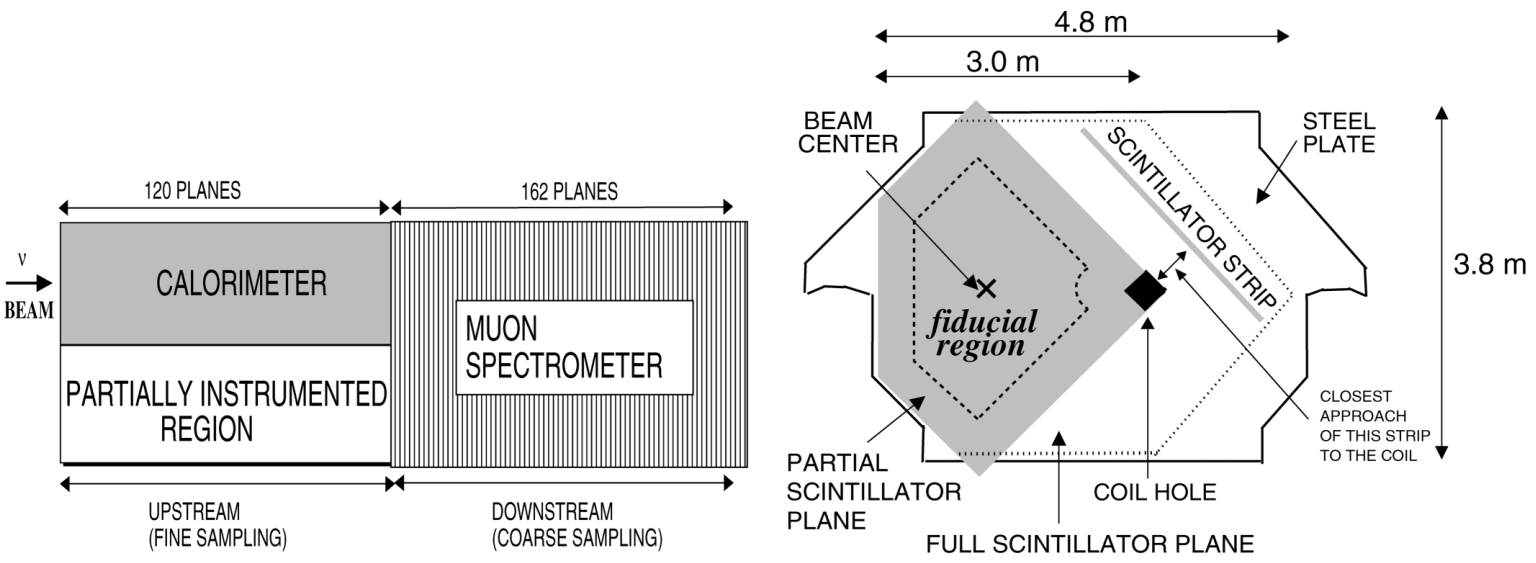
\includegraphics[width=0.9\textwidth]{plots/minos.png}
	\caption{Left: Top view of the MINOS near detector, showing the calorimeter and muon spectrometer (not to scale). Right: transverse view of a near detector plane. The shaded area shows a partially instrumented active scintillator plane and the dashed line within shows the boundary of the fiducial region. The dotted line shows the outline of a fully instrumented scintillator plane. Reproduced from Figure~2 of~\cite{MINOSDetectors}.}
	\label{fig:minos_near_detector}
\end{figure}

As the majority of muons are not contained within the MINERvA volume, and mostly exit downstream, MINERvA currently employ MINOS as a muon spectrometer. Similarly, for ProtoDUNE-ND, the majority of particles will not be contained in the ArgonCube 2x2 volume. Even if MINERvA components are placed downstream of the 2x2 module, the majority of muons will not be contained, making ancilliary physics measurements with ProtoDUNE-ND extremely challenging. Employing MINOS ND as a range finder for ProtoDUNE-ND would allow the muon momentum to be measured, and would allow ProtoDUNE-ND to make much more DUNE-ND-like measurements. If MINOS-ND were to be included downstream, of the MINERvA component, it would also make sense to deploy portions of the MINERvA detector around the ArgonCube cryostat, since the entire MINERvA detector would no longer be needed downstream to maximize momentum sensitivity, making it much easier to tag escaping particles, and to identify through-going cosmics (as alluded to in Section~\ref{sec:cosmic-suppression}), which would make is much easier to calibrate the energy scale in the detector. MINERvA EM scintillator modules could be used to provide vetos for cosmic and rock induced particles entering or exiting the 2x2 cryostat, or to contain side-escaping showers. Ultimately, this would enable a test of the assumption that the DUNE ND does not require a side muon tracker.

Here we discuss such possibilities in brief, and will wait to discover the viability of this project before embarking on more detailed studies. Use of the MINOS ND, in combination with an augmented MINERvA, would allow the reconstruction of the entire properties of an event which occurred in the ArgonCube 2x2 volume. This serves as a proxy for neutrino energy reconstruction, as it would in the full DUNE-ND, and would provide the most thorough calibration of the response of 2x2 possible --- vital, as there are no plans to calibrate the response in a test beam before installation in the MINOS-ND hall at Fermilab.

\subsubsection{Validation of multiple coulomb scattering}

The DUNE ND will employ a downstream tracking detector to measure forward, high-energy muons, and will be sufficiently wide as to contain muons at high angles.  However, for wide-angle muons, tracks will only be contained when the vertex is far from the edges, and will often exit the TPC and not be reconstructed.  This sample could be recovered if the muon momentum can be measured reliably from multiple coulomb scattering (MCS). The far detector will also use MCS for muons which exit the detector.

Such measurements have been carried out in a LAr TPC by MicroBooNE~\cite{Abratenko:2017nki}, although the momentum range is somewhat limited as the only validation sample available is composed of muons which stop in the detector, for which a momentum by range measurement can be made. However, such measurements may be more challenging in a modular TPC such as ArgonCube, where tracks are necessarily broken into segments which are read out separately, and then combined in downstream software.

Although there are only four modules in the ArgonCube 2x2 Demonstrator, each is split into two TPCs, so tracks which exit the downstream face of the 2x2 module may be sampled by up to four independent charge readout planes. With a downstream detector capable of making a precise muon momentum measurement, it would be possible to demonstrate that multiple coulomb scattering will be a viable technique for making momentum measurements in the full ArgonCube deployment in the DUNE ND. Given the hard muon momentum spectrum expected in the NuMI on-axis beam (shown in Figure~\ref{fig:momenta}), it would be hard to make a reliable momentum measurement with a small demonstrator tracker module, or indeed with the MINERvA components proposed in Section~\ref{sec:minerva}, as few would be contained. Such measurements could be made, in the MINOS-ND, which is capable of making momentum measurements for all relevant muon momenta by curvature, or by range.

\subsubsection{Use of MINERvA as a cosmic trigger}
In the discussion in Section~\ref{sec:minerva}, the detector setup maximizes the amount of the MINERvA detector repurposed downstream of the ArgonCube 2x2 module, in order to increase containment in the very forward region, where most particles go. However, if MINOS-ND is also included as part of the ProtoDUNE-ND setup, this imperative is no longer there, and less of MINERvA would be needed downstream. In this case, MINERvA modules could be redeployed to the sides of, and even above, the 2x2 cryostat to act as a cosmic ray or dirt muon tagger, and to tag escaping particles. In practice, these panels could be used to better identify a sample of fully contained neutrino events for the studies outlined in Sections~\ref{sec:minerva-acceptance}. Additionally, these cosmic ray tagging modules could then be used to validate space charge build-up and electric field uniformity studies outlined in Section~\ref{sec:efield}, and the cosmic suppression studies described in Section~\ref{sec:cosmic-suppression}, for which an additional scintillator panel would be required.

